%
% File acl2019.tex
%
%% Based on the style files for ACL 2018, NAACL 2018/19, which were
%% Based on the style files for ACL-2015, with some improvements
%%  taken from the NAACL-2016 style
%% Based on the style files for ACL-2014, which were, in turn,
%% based on ACL-2013, ACL-2012, ACL-2011, ACL-2010, ACL-IJCNLP-2009,
%% EACL-2009, IJCNLP-2008...
%% Based on the style files for EACL 2006 by 
%%e.agirre@ehu.es or Sergi.Balari@uab.es
%% and that of ACL 08 by Joakim Nivre and Noah Smith

\documentclass[11pt,a4paper]{article}
\usepackage[hyperref]{acl2019}

\usepackage{times}
\usepackage{latexsym}
\usepackage{amsmath}
\usepackage{amssymb}
\usepackage{graphicx}
\usepackage[utf8x]{inputenc}
\usepackage{url}
\usepackage{multirow}
\usepackage{enumitem}
\newcommand{\KZ}[1]{\textcolor{blue}{Kenny: #1}}

%\aclfinalcopy % Uncomment this line for the final submission
\def\aclpaperid{1109} %  Enter the acl Paper ID here

%\setlength\titlebox{5cm}
% You can expand the titlebox if you need extra space
% to show all the authors. Please do not make the titlebox
% smaller than 5cm (the original size); we will check this
% in the camera-ready version and ask you to change it back.

\newcommand\BibTeX{B{\sc ib}\TeX}

\title{Unsupervised Multilingual Contextualized Representations for Low-Resource Sequence Labeling}

\author{First Author \\
	Affiliation / Address line 1 \\
	Affiliation / Address line 2 \\
	Affiliation / Address line 3 \\
	{\tt email@domain} \\\And
	Second Author \\
	Affiliation / Address line 1 \\
	Affiliation / Address line 2 \\
	Affiliation / Address line 3 \\
	{\tt email@domain} \\}

\date{}

%\hypersetup{draft} %for bug

\begin{document}
	\maketitle
	\begin{abstract}
		Previous work on cross-lingual sequence labeling tasks either requires parallel data or bridges the two languages through word-by-word matching. Such requirements and assumptions are infeasible for most languages, especially for languages with large linguistic distances, e.g., English and Chinese.
		In this work, we propose a Multilingual Language Model with deep semantic Alignment (MLMA) to generate language-independent representations for cross-lingual sequence labeling. 
		Our methods require only monolingual corpora with no bilingual resources at all and take advantage of deep contextualized representations in
		addition to word-level alignment.
        Experimental results show that our approach achieves new state-of-the-art NER and POS performance across European languages, and is also effective on distant language pairs such as English and Chinese.
	\end{abstract}
	
	%\setlength{\abovedisplayskip}{3pt}
	%\setlength{\belowdisplayskip}{3pt}
	\section{Introduction}
	Sequence labeling tasks such as named entity recognition (NER) and part-of-speech (POS) tagging are fundamental problems in natural language processing (NLP). Recently, neural sequence labeling models achieve state-of-the-art performance by combining both character-level and word-level information~\cite{chiu16named,ma16end,lample16neural}. However, these neural models heavily rely on large-scale annotated training data, which may not be available in most languages.
	
	Cross-lingual transfer learning is proposed to address the label scarcity problem by transferring models learned from high-resource languages (source languages) to low-resource languages (target languages). In this scenario, a major challenge is how to bridge interlingual gaps with modest resource requirements.
	
	%\newcite{McDonald11multi} and \newcite{tackstrom12cross} utilize a manually designed universal POS tagset as language-independent features to train a cross-lingual parser. In the field of NER, morphological features, such as word forms, affixes, and capitalization, are regarded invariant between similar languages~\cite{tsai16cross}.
	
	%There is a large body of work exploring cross-lingual transfer through language-independent feature engineering. 
	There is a large body of work exploring cross-lingual transfer through language-independent features, such as morphological features and universal POS tags for cross-lingual NER~\cite{tsai16cross} and dependency parsers~\cite{McDonald11multi}. However, these approaches require linguistic knowledge for language-independent feature engineering, which is expensive in low-resource settings. Other work relies on bilingual resources to transfer knowledge from source languages to target languages. Parallel corpora are widely used to project annotations from the source to the target side~\cite{yarowsky2001inducing,ehrmann11building,kim12multilingual,wang14cross}. These methods could achieve strong performance with a large amount of bilingual data, which is scarce in low-resource settings. 
	
	Recent research in cross-lingual transfer learning leverages cross-lingual word embeddings (CLWEs) to establish inter-lingual connection~\cite{ni17weakly,fang2017model,xie2018neural}. 
	%CLWEs not only shifts the burden of expensive language-independent feature engineering, but also require just small bilingual lexicons or even no bilingual supervised resources~\cite{artetxe16learning,conneau2017word}.
	CLWEs reduce the requirements of feature engineering and parallel data to only a small bilingual lexicon or even no bilingual resource~\cite{artetxe16learning,conneau2017word}. However, word embedding spaces may not be completely isomorphic due to language-specific linguistic properties, and therefore cannot be perfectly aligned. For example, different from English, Chinese nouns do not distinguish between singular and plural forms, while Spanish nouns distinguish masculine and feminine. In this work, we assume that the semantic meanings of words from different languages can be roughly aligned at a conceptual level. This assumption motivates us to align deep semantic representations instead of shallow word embeddings. Meanwhile, monolingual contextualized embeddings derived from language models have shown to be effective for extracting semantic information and have achieved significant improvement on several NLP tasks~\cite{peters2018deep}. Thus, we employ language models to generate contextualized representations and propose three methods to align them across languages.
	
	In this paper, we propose a Multilingual Language Model with deep semantic Alignment (MLMA). We train MLMA on monolingual corpora from each language and align its internal states across different languages. Then MLMA is utilized to generate language-independent representations and to bridge the gaps between high-resource and low-resource languages. For evaluation, we conduct extensive experiments on the NER and POS benchmark datasets under cross-lingual settings. The experiment results show that our methods achieve substantial improvements comparing to previous state-of-the-art methods in European languages. We also validate our approaches on a distant language pair, English-Chinese, and our results are competitive with previous methods which use large-scale parallel corpora. Our contributions are summarized as follows:% To the best of our knowledge, we are the first work to align cross-lingual contextualized representations in the context of language models.
	%\vspace{-0.5em}
	\begin{enumerate}\setlength{\itemsep}{-0.1cm}%[itemsep=0mm]
		\item Instead of word-level alignment, we propose MLMA that uses contextualized representations to bridge the inter-lingual gaps.
		\item We propose three methods to align contextualized representations without any bilingual resource.
		\item Our methods achieve new state-of-the-art performance on cross-lingual NER and POS tasks in European languages, and very competitive results for English-Chinese NER, where previous work uses a large amount of parallel data.
	\end{enumerate}
	
	\section{Approach}
	The architecture of MLMA is shown in Figure~\ref{fig:main_architecture}. Our approach belongs to the model transfer group (Section~\ref{sec:model_transfer}) and mainly consists of three steps:
	%\vspace{-0.5em}
	\begin{enumerate}\setlength{\itemsep}{-0.1cm}
	\item Training a multilingual language model with alignment (MLMA) using monolingual corpora of both the source and the target languages.
	\item Building a cross-lingual sequence labeling model based on the language-independent representations from the MLMA. %extracted from multilingual language model.
	\item Learning the cross-lingual sequence labeling model on the annotated data of source languages and directly applying it to the target languages. 
	\end{enumerate}
	
    In the following sections, we first present the architecture of MLMA and describe how to build the unsupervised multilingual alignment. Next, we propose effective methods for collapsing the multi-layer hidden states from MLMA into a single representation. Finally, we introduce the architecture of the sequence labeling model used in the experiments.

	\subsection{Language Model Architecture}
	\begin{figure*} 
		\centering
		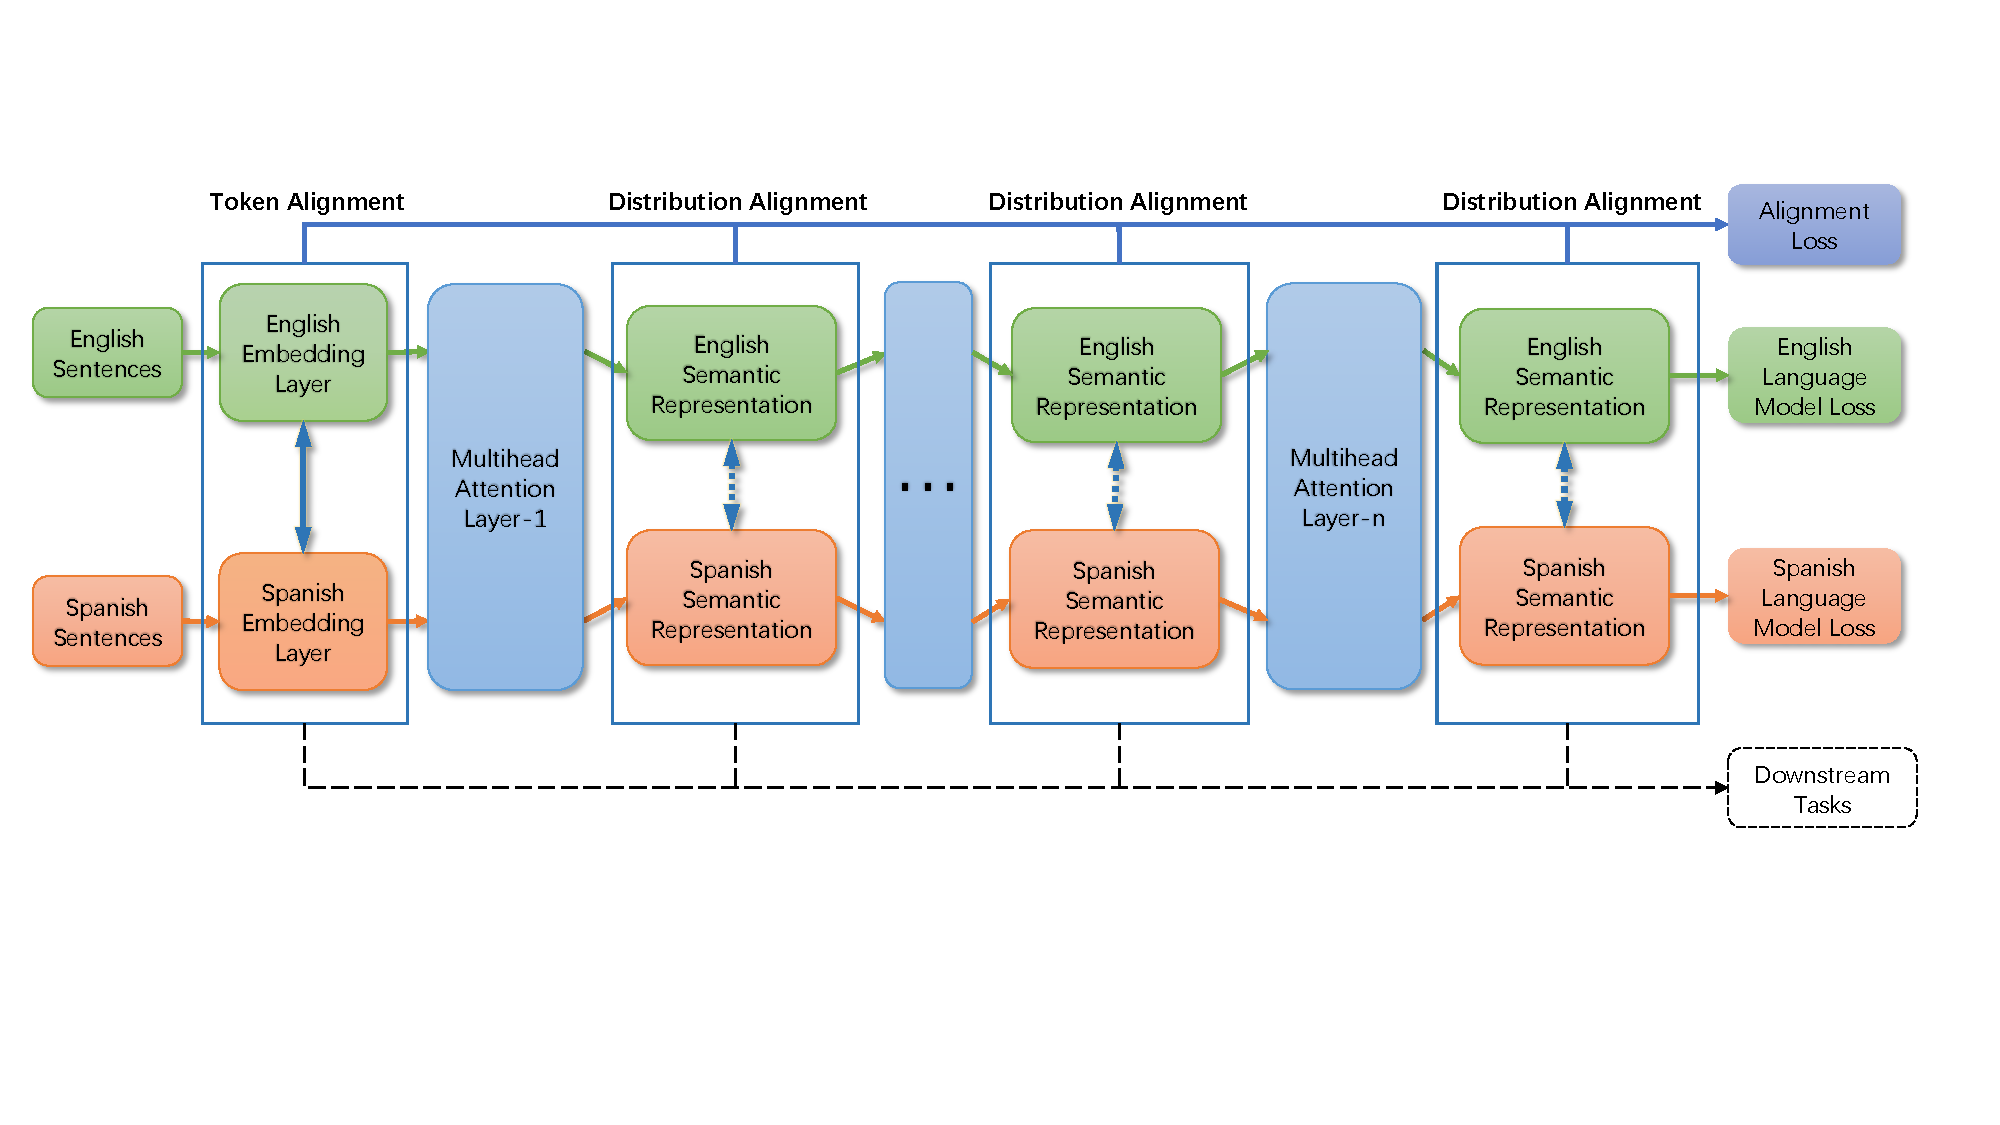
\includegraphics[trim=0.5cm 5cm 1.3cm 3cm,clip,width=1.0\textwidth]{architecture2.pdf}
		\caption{The architecture of MLMA, which consists of language-specific embedding layers and language-agnostic Transformer layers. MLMA is jointly learned through the language modeling loss and alignment loss, and its internal representations are utilized to bridge the gap between source and target languages. }
		%\vspace{-2em}
		\label{fig:main_architecture}
	\end{figure*}
	MLMA is a Transformer language model with multi-head self-attention mechanism~\cite{vaswani2017attention}. The architecture is similar to \newcite{radford2018improving}, except that we combine both a forward and a backward Transformer decoder to build a bidirectional language model. Take the forward direction as an example, given a sentence with $N$ tokens $W = [w_1, w_2, \cdots, w_N]^T$ as input, we first map the sequence of tokens $W$ to token embeddings $\overrightarrow{H}_0 \in \mathbb{R}^{N \times d} $:
	\setlength{\abovedisplayskip}{3pt}
	\setlength{\belowdisplayskip}{3pt}
	\begin{equation}
	%\small
	\overrightarrow{H}_0 = WE_e + E_p
	\end{equation}
	where $E_e$ and $E_p$ are the embedding matrix and the positional encoding matrix, and $d$ is the dimension of embeddings and hidden states.
	
	Then $n$ blocks of transformer layers are stacked above the token embeddings. Each block contains a multi-head self-attention and a position-wise feedforward layer. The detailed implementation is the same as~\cite{vaswani2017attention}.
	\begin{equation} \label{eq:transformer_layer}
	%\small
	%  \begin{aligned}
	\overrightarrow{H}_l = {\rm TransformerLayer}(\overrightarrow{H}_{l-1})%, \ \ \forall l \in [1, n] 
	%  \end{aligned}
	\end{equation}
	Finally the output distribution over next tokens are calculated through a softmax function with tied embedding matrix.
	\begin{equation}
	%\small
	\overrightarrow{P} = {\rm softmax}(\overrightarrow{H}_n E_e^T)
	\end{equation}
	For the backward direction, we calculate $\overleftarrow{H_l}$ and $\overleftarrow{P}$ in an analogous way. Finally, we jointly minimize the negative log likelihood of the forward and backward directions:
	\begin{equation} \label{eq:NLL}
	%\small
	\begin{aligned} 
	NLL = - \sum_{t=1}^N (&\log p(w_t | w_1, \ldots, w_{t-1}) \\
	+ &\log p(w_t | w_{t+1}, \ldots, w_{N}))
	\end{aligned}
	\end{equation}
	%Our language model architecture is similar to \cite{radford2018improving}, except that we combine both a forward and a backward Transformer decoder to build a bidirectional language model. 
	
	In a multilingual setting, we share all parameters in Transformer layers across different languages to facilitate language-agnostic representations, except that we adopt an individual embedding matrix $E_e$ for each language.
	
	\subsection{Unsupervised Distribution Alignment}
	
	We find that only sharing Transformer layers is not enough for forcing hidden representations from different languages into a common space, as suggested in experiments (Section~\ref{sec:result_ner}). Therefore, we propose three methods to build cross-lingual representations based on identical strings, mean/variance, and average linkage.
	
	To simplify the description, we take the alignment between two languages $s$ and $t$ as an example, but our methods can be directly extended to a scenario with multiple languages by adding the alignment between each pair of languages.
	
	\subsubsection*{Notation}
	For the language model, given a sentence with $N$ tokens, the forward internal representation  $\overrightarrow{H}_l$ in Eq~\eqref{eq:transformer_layer} can be expanded as $\overrightarrow{H}_l = [\overrightarrow{h}_{l,1}, \cdots, \overrightarrow{h}_{l,k}, \cdots, \overrightarrow{h}_{l,N}]^T$, where $\overrightarrow{h}_{l,k}$ refers to the forward hidden representation of the $k$-th token in the sentence. Then we concatenate the forward and backward hidden representations for each token, $h_{l,k} = \overrightarrow{h}_{l,k} \oplus \overleftarrow{h}_{l,k}$.
	
	We denote the collection of the token representations at layer $l$ from the whole corpora of language $s$ as $C_l^s$, which can be regarded as a sampling from the deep semantic space of language $s$. Similarly, $C_l^t$ is used for language $t$.
	
	\subsubsection*{Identical Strings}
	Similar language pairs such as English and Spanish have a large number of identical strings shared between their vocabularies, which are utilized as the seed dictionary for embedding alignment in previous work~\cite{smith2017offline}. Similarly, we treat identical strings as explicit supervision signals and align the embeddings of identical strings between different languages. %Since we adopt a softmax function with tied embedding matrices at the output layer, the alignment of both ``input" and ``output" will lead to a further matching of inner states. 
	In the experiments, we directly minimize the Euclidean distance between the embeddings of each identical string across different languages:
	\begin{equation*}
	%\small
	L_{id} = \dfrac{\lambda^{id}}{| W_{id}^{(s,t)} |} \sum_{w \in W_{id}^{(s,t)}} ||e_{w}^s - e_{w}^t||
	\end{equation*}
	where $W_{id}^{(s,t)}$ is the set of identical strings between language $s$ and language $t$, and $|W_{id}^{(s,t)}|$ refers to the number of members in $W_{id}^{(s,t)}$. $\lambda^{id}$ is a scaling weight, and $e_{w}^s$ ($e_{w}^t$) is the embedding of word $w$ from embedding matrix $E_e^s$ ($E_e^t$). 
	
	%Different from an offline linear projection~\cite{mikolov2013exploiting}, we dynamically update embeddings of MLMA during the process of language modeling. 
	
	The matching of the embeddings of identical strings from different languages will lead to an implicit alignment of internal representations. 
	
	\subsubsection*{Mean and Variance}
	%In a cross-lingual setting, we desire the internal semantic representation to be shared and therefore generalized well across different languages. 
	In this section, we propose another approach to directly align the distributions of internal representations between different languages at each layer. In particular, we leverage the mean and variance of internal distributions for alignment. We denote the mean and variance of $C_l^s$ as $m_{l}^s$ and $v_{l}^s$. Similarly, $m_{l}^t$ and $v_{l}^t$ refer to the mean and variance of $C_l^t$. We minimize the Euclidean distance between the mean and variance of language $s$ and language $t$ for all layers:
	\begin{equation*}
	%\small
	L_{mv} = \sum_{l=0}^n (\lambda_{l}^m \cdot \dfrac{||m_{l}^s - m_{l}^t||}{|m_{l}^s| + |m_{l}^t|} + \lambda_{l}^v \cdot \dfrac{||v_{l}^s - v_{l}^t||}{|v_{l}^s| + |v_{l}^t|})
	\end{equation*}
	where $\lambda_{l}$ is a scaling weight, and $|\cdot|$ is the L1 norm of a vector. Without the denominators, the model could escape this regularization by learning a mean and variance with low absolute values.
	%The denominators are used to prevent the model from escaping this regularization loss. Without the denominators, the mean and variance could end up with low absolute values.
	
	In practice, rather than calculating the mean and standard deviation over the whole source and target corpora, we only calculate and align them inside the mini-batch as an approximation.
	
	\subsubsection*{Average Linkage}
	%Apart from the mean and variance
	In this method, we employ another metric, average linkage, to perform a more precise point-wise matching. The average linkage measures the similarity of two sets $X$ and $Y$ by calculating the averaged distance between all members of each set:
	\begin{equation*}
	%\small
	avl(X, Y) = \dfrac{1}{n_{X} \cdot n_{Y}} \sum_{x \in X} \sum_{y \in Y} f(x, y)
	\end{equation*}
	where $n_X$ ($n_Y$) is the number of members in $X$ ($Y$), and $f$ is a distance function. We take Euclidean distance as the distance function $f$ and minimize the average linkage between $C_l^s$ and $C_l^t$:
	\begin{equation*}
	%\small
	\begin{aligned}
	L_{avl} = \sum_{l=0}^n & \lambda_{l}^{avl} \cdot [2 \cdot avl(C_l^s, C_l^t) \\
	& - avl(C_l^s, C_l^s)  - avl(C_l^t, C_l^t)]
	\end{aligned}
	\end{equation*}
	Similarly, the terms $avl(C_l^s, C_l^s)$ and $avl(C_l^t, C_l^t)$ are used to prevent the model from escaping this regularization. In practice, we only calculate $L_{avl}$ inside the mini-batch as an approximation.
	
	The regularization $L_{avl}$ is similar to the maximum mean discrepancy (MMD), which is often employed in domain adaptation~\cite{tzeng2014deep,long2015learning} and style transfer~\cite{li2017demystifying} for images. However, different from MMD, our method directly uses Euclidean distance instead of the kernel function.
	
	\subsection{Training of MLMA}
	During the training stage of MLMA, we sample equivalent number of sentences from the monolingual corpora of each language for each mini-batch. Then MLMA is optimized through a combination of the language modeling loss $L_{lm}$ and the alignment regularization loss $L_{reg}$. For each alignment method, we use its corresponding alignment loss:
	\begin{equation*}
	%\small
	\begin{aligned}
    L = &L_{lm} + L_{reg} \\
	{\rm where}\ \ &L_{lm} =  \sum_{i \in \{s, t\}} \lambda_{i}^{lm} \cdot NLL_i, \\
	&L_{reg} \in \{L_{id}, L_{mv}, L_{avl}\}
	\end{aligned}
	\end{equation*}
	where $\lambda_{i}^{lm}$ is the hyperparameter for balancing the convergence speed between different languages. $NLL_i$ is the negative log likelihood of language $i$ in Eq~\eqref{eq:NLL}.
	
	\subsection{Cross-lingual Contextualized Representations}
	We extract the hidden states from the MLMA as cross-lingual contextualized representations (CLCRs). However, integrating these multi-layer high-dimensional embeddings into downstream models is not straightforward. In this section, we propose two effective strategies:
	
	\noindent\textbf{Self-Weighted Sum} For each token, we concatenate all layers of hidden states and feed them into a multi-layer perceptron (MLP) to calculate a $(n+1)$-dimensional weight vector, $s = {\rm softmax}({\rm MLP}(h_{0,k} \oplus \cdots \oplus h_{n,k}))$. Then we calculate a weighted sum of these layers according to the weight vector, $\textbf{CLCR}_k = \sum_{l=0}^n s_{l}\cdot h_{l,k}$.
	
	\noindent\textbf{Fully-Weighted Sum} We introduce a weight matrix, $F \in \mathbb{R}^{(n+1) \times 2d}$, with separate weights for each hidden dimension. The weight matrix $F$ is softmaxed by column and used to calculate a weighted sum of all layers for each hidden dimension, $\textbf{CLCR}_k = \sum_{l=0}^n F_l \odot h_{l,k}$, where $\odot$ is the element-wise product.
	
	%\textbf{Gate-Weighted Sum (GWS)} Similar to FWS, except that the weight matrix is calculated from an affine transformation followed by a non-linearity $\textbf{w} = \sigma (\textbf{h}_k\textbf{T} + \textbf{b})$ where \textbf{T} is a $D \times D$ square matrix.
	The parameters of the ${\rm MLP}$ and $F$ are trained during the learning of sequence labeling model.
	%Intuitively, Self-Weighted Sum allows weights to adapt to each position in a sequence, while Fully-Weighted Sum allows weights to adapt to each hidden dimension.
	
	%In the experiments, we directly use \textbf{CLCR}s as pre-trained embeddings in the sequence labeling model without concatenating any other pre-trained word vectors such as GloVe or fastText~\cite{pennington2014glove,bojanowski2017enriching}.
	
	\subsection{Sequence Labeling Model}
	We briefly introduce the sequence labeling model used in this work. For both NER and POS tasks, we use an LSTM-CRF model largely following \cite{lample16neural}, which consists of a character-level LSTM, a word-level LSTM, and a linear-chain CRF. 
	
	More specifically, given a sequence of words as $[w_1, w_2, \ldots, w_N]$, where $w_k$ is composed of a sequence of characters $[c_{k,1}, c_{k,2}, \ldots, c_{k,m}]$. First, for each word $w_k$, the character-level LSTM takes its character sequence $[c_{k,1}, c_{k,2}, \ldots, c_{k,m}]$ as input and outputs a vector $e_k$ to represent this word. Then the pre-trained $\textbf{CLCR}_k$ is concatenated with $e_k$ to form a word-level embedding $x_k$. Finally, the sequence of word-level embeddings $[x_1, x_2, \ldots, x_N]$ are fed into the word-level LSTM, and the linear-chain CRF are employed to predict the probability distribution for all possible output label sequences.
	
	%The sequence of word-level embeddings $[x_1, x_2, \ldots, x_N]$ are fed into the word-level LSTM to generate a  sequence of hidden representations $(r_1, r_2, \ldots, r_N)$, which are finally calculated in the linear-chain CRF to predict a probability distribution for all possible tag sequences.
	
	\section{Experiments}

	We first introduce the datasets used in the experiment and
	then the implementation details of our models, before presenting the results on NER and POS tasks. 

	\subsection{Datasets} 
	For cross-lingual NER, we evaluate the proposed approaches on CoNLL 2002/2003 datasets~\cite{tksintro2002conll,tjongkimsang2003conll}, which contain four European languages, English (en), Spanish (es), Dutch (nl), German (de). We also evaluate a distant language pair, English-Chinese, on OntoNotes(v4.0) dataset~\cite{hovy2006ontonotes}, and follow the same dataset split and entity types as described in \cite{wang14cross}.
	%English is used as the source language, and the other three are used as target languages. 
	
	For cross-lingual POS, we use the Danish (da), Dutch (nl), German (de), Greek (el), Italian (it), Portuguese (pt), Spanish (es) and Swedish (sv) portion from CoNLL 2006/2007 dataset~\cite{buchholz2006conll,nivre07the} and adopt the universal POS tagset~\cite{petrov11auniversal}.
	
	In all cases, the sequence labeling model is trained on the source language (English) training data and is tested on the target language test data.
	
	%. In the experiment, we adopt the universal POS tagset~\cite{petrov11auniversal} for all languages.%Following previous work, we train the sequence labeling model on Penn Treebank data and make use of the last 20 sentences in target language training data for development purposes. %We train an English POS tagger on Penn Treebank data as source sequence labeling model and make use of the last 20 sentences in target language training data for development purposes. In the experiment, we adopt the universal POS tagset~\cite{petrov11auniversal} for all languages.
	
	% The hyperparameter settings of our multilingual language modeling largely follows the original transformer decoder~\cite{vaswani2017attention}.
	\subsection{Details of MLMA}  
	We adopt a 6-layer bi-directional Transformer decoder with 8 attention heads. The dimension size of hidden states and inner states are 512 and 2048, respectively. The dropout rates after attention and residual connection are both 0.1. We use the Adam optimization scheme~\cite{kingma2014adam} with a learning rate of 0.0001 and train the model with a sampled softmax~\cite{jean15on} of 8192 samples. Each batch contains around 4096 tokens for each language. The language modeling weight $\lambda_i^{lm}$ is set to be 1.0 for each language. For alignment, $\lambda_l^m$, $\lambda_l^v$, $\lambda_l^{al}$ are set to be 0.1, 0.01 and 1.0 for every layer $l$, and $\lambda^{ide}$ is set to be 100.
	
	% and a gradient clip norm of 5.0. The vocabulary size of each language is 200,000,
	%Spanish, Dutch, German, Chinese, Danish, Greek, Italian, Portuguese and Swedish
	For languages except English, the latest dump of Wikipedia\footnote{\url{https://dumps.wikimedia.org/}} is used as monolingual corpora. For English, we use 1B Word Benchmark~\cite{chelba2013one} to reduce the effects of potential internal alignment in Wikipedia~\cite{zirikly15cross,tsai16cross}. 
	
	%All characters are preprocessed to lowercase, and Chinese are converted into simplified version through OpenCC\footnote{\url{https://github.com/BYVoid/OpenCC}}. The corpora of European languages are tokenized by nltk~\cite{loper2002nltk} and Chinese text is segmented using Ltp\footnote{\url{https://github.com/HIT-SCIR/pyltp}}.
	
	\subsection{Details of Sequence Labeling Model} 
	The size of character embedding, word-level LSTM, and character-level LSTM are set to be 100, 300 and 100, respectively. We train the sequence labeling model for 20 epochs using Adam optimizer with a batch size of 20 and perform an early stopping when there is no improvement for 3 epochs. For each model, we run it five times and report the mean and standard deviation. We disable the character-level LSTM in English-German and English-Chinese NER as they have a different character pattern from English. For POS, we disable the character-level LSTM following~\cite{fang2017model}.
	%We apply dropout at both the input and the output of word-level LSTM to prevent overfitting. The dropout rate is set to be 0.5. 
	%We train the sequence labeling model for 20 epochs using Adam optimizer with a batch size of 20 and perform an early stopping when there is no improvement for 3 epochs on the target language development dataset. We set the initial learning rate to be 0.001 and decay the learning rate by 0.1 for each epoch. We do not update the pre-trained cross-lingual deep representations from MLMA during training. For each model, we run it five times and report the mean and standard deviation.% of the results.
	
	%We observe that the character patterns of some languages are different from English. For instance, all nouns in German are capitalized, and Chinese has a distinct alphabet. Therefore, we disable the character-level LSTM in English-German and English-Chinese NER.
	%For cross-lingual POS, we disable the character-level LSTM following~\cite{fang2017model}.%, and an earlier experiment indicated that adding a character-level LSTM does not improve the performance.
	
	
	\subsection{Results for NER} \label{sec:result_ner}
	\begin{table*}[th]
		\small
		\centering
		\begin{tabular}{l c c c l} 
			Model  &  es & nl & de & Extra Resources\\
			\hline
			MLM (w/o alignment) + s.w.s. & 21.16 ± 1.40 & 33.97 ± 1.49 & 15.46 ± 1.21 & None\\
			MLM (w/o alignment) + f.w.s. & 23.61 ± 2.33 & 32.94 ± 1.62 & 16.38 ± 1.09 & None\\
			\hline
			\newcite{tackstrom12cross} & 59.30 & 58.40 & 40.40 & parallel corpus\\
			\newcite{nothman13learning} & 61.00 & 64.00 & 55.80 & Wikipedia\\
			\newcite{wang14cross} & - & - & 60.00 & parallel corpus\\
			\newcite{tsai16cross} & 60.55 & 61.60 & 48.10 & Wikipedia\\
			\newcite{ni17weakly} & 65.10 & 65.40 & 58.50 & Wikipedia, parallel corpus, 5K dict.\\
			\newcite{mayhew17cheap} & 65.95 & 66.50 & 59.11 & Wikipedia, 1M dict.\\
			\newcite{xie2018neural} & 72.37 & 71.25 & 57.76 & None\\
			MUSE* & 66.17 ± 1.15 & 65.52 ± 0.78 & 55.46 ± 0.59 & None\\
			\hline
			%\textit{Our methods} & & & &\\% & \\
			MLMA-Iden + s.w.s. & 69.45 ± 0.91 & 68.82 ± 0.82 & 55.75 ± 1.64 & None\\
			MLMA-Iden + f.w.s. & 67.10 ± 0.78 & 68.15 ± 0.67 & 55.25 ± 1.29 & None\\
			MLMA-Mv + s.w.s. & 73.81 ± 0.83 & 70.61 ± 1.79 & 57.70 ± 0.71 &  None\\
			MLMA-Mv + f.w.s. & 74.12 ± 1.00 & 71.72 ± 0.70 & 57.84 ± 0.80 &  None\\
			MLMA-Avl + s.w.s. & 75.01 ± 0.79 & 76.22 ± 0.42 & 60.98 ± 1.00 & None \\
			MLMA-Avl + f.w.s. & 74.43 ± 0.50 & 76.02 ± 0.55 & 60.50 ± 0.43 & None \\
			%Token + Layer Align AL + SA & 75.30 ± 0.64 & 76.29 ± 0.81 & 62.74 ± 0.31 & None\\
			MLMA-Avl (init) + s.w.s. & 75.72 ± 0.80 & \textbf{76.90} ± 0.30 & 63.01 ± 0.83 & None\\
			MLMA-Avl (init) + f.w.s. & 76.30 ± 0.76 & 76.85 ± 0.43 & 62.85 ± 0.47 & None\\
			MLMA-Avl (multi) + s.w.s. & \textbf{79.36} ± 0.57 & 74.89 ± 0.28 & 65.93 ± 0.32 & None\\
			MLMA-Avl (multi) + f.w.s. & 79.34 ± 0.35 & 74.74 ± 0.40 & \textbf{66.53} ± 0.35 & None\\
			\hline
		\end{tabular}
		%\caption{ Test performance of cross-lingual NER on CoNLL. For previous work who reports multiple results, we only list their best performance on each language. Results of methods with mark * are obtained by re-running the released source code on our monolingual corpora.}
		\caption{ NER F1 scores on test sets of European languages. For previous work which reports multiple results, we only list their best performance on each language. Results of methods with mark * are obtained by running their released source code. The results of MUSE embeddings are produced by using them for direct model transfer. ``MLM" denotes our multilingual language model without alignment. ``Iden", ``Mv" and ``Avl" refer to the alignment methods of identical vocabularies, mean/variance and average linkage, respectively. ``s.w.s" and ``f.w.s." are self-weighted sum and fully-weighted sum. ``init" represents using MUSE to initialize the embedding matrices in the MLMA. ``multi" refer to the multi-source transfer.}
		\vspace{-1em}
		\label{table:NERmain}
	\end{table*}
	
	We first train a multilingual language model without alignment (MLM) and report its performance in cross-lingual NER. As shown in Table~\ref{table:NERmain}, the poor performance demonstrates that only sharing parameters in a multilingual language model is far from enough for cross-lingual alignment.
	
	%Previous work (see Section \ref{sec:related}) utilizes extra bilingual resources to build the interlingual connection. 
	As shown in Table~\ref{table:NERmain}, the mean/variance alignment strategy (MLMA-Mv) is competitive with previous work which utilizes extra bilingual resources (Section \ref{sec:annotation_projection}). The average linkage strategy (MLMA-Avl) performs a more precise alignment and gains a further improvement.% over other approaches. 
	
	To demonstrate the strengths of the proposed cross-lingual contextualized representations (CLCRs) over cross-lingual word embeddings (CLWEs), we also report the results of using CLWEs for direct model transfer in Table~\ref{table:NERmain}.  Specifically, we use the unsupervised method MUSE~\cite{conneau2017word} to generate CLWEs for each language pair. The experiment results demonstrate its effectiveness for cross-lingual sequence labeling. The alignment method using identical strings (MLMA-Iden) outperforms MUSE, suggesting that the contextual-level representations are more effective than the word-level ones. The other proposed methods (MLMA-Mv and MLMA-Avl) achieve significant improvement over MUSE embeddings and the token-level alignment approach, which shows the benefit of directly aligning the contextualized representations.
	
	\noindent\textbf{Combination with CLWEs} We further demonstrate that CLWEs are compatible with our methods by using MUSE embeddings to initialize the embedding layer of our multilingual language model. The results of MLMA-Avl (init) shown in Table~\ref{table:NERmain} indicate that the CLWEs lead to a better initialization and improved performance.
	
	\noindent\textbf{Multi-source Transfer} We conduct experiments of multi-source transfer based on method MLMA-Avl and report the performance as MLMA-Avl (multi) in Table~\ref{table:NERmain}. For Spanish and German, we use English and Dutch as source languages. English and Spanish are adopted for Dutch. The multi-source transfer leads to a significant improvement for Spanish and German, but a slight decline for Dutch. In the follow-up experiment, we find that the Spanish training set achieves a poor cross-lingual performance on Dutch. Similar results are observed on the experiments of Spanish to English and Dutch to English. These results suggest that the cross-lingual transfer may be directional, and we leave this issue for future work.
	
	%To explain the performance decline, we train a NER model with the Spanish training set only and find that this model achieves a poor cross-lingual performance on the Dutch development set.
	
	\begin{table}[t]
		%\small
		\centering
		\begin{tabular}{l c} 
			Model  & zh \\
			\hline
			\newcite{wang14cross}$\diamond$ & \textbf{64.40} \\
			MUSE* & 35.35 ± 0.84 \\
			\newcite{xie2018neural}* & 44.13 ± 1.49 \\
			\hline
			\textit{Our methods} & \\
			MLMA-Iden + s.w.s. & 11.08 ± 0.89 \\
			MLMA-Iden + f.w.s. & 11.17 ± 0.69 \\
			MLMA-Avl + s.w.s. & 50.11 ± 1.51 \\
			MLMA-Avl + f.w.s. & 45.88 ± 2.49 \\
			%Token + Layer Align AL + SA & 53.41 ± 0.78 \\
			MLMA-Avl (init) + s.w.s & 60.33 ± 1.39 \\
			MLMA-Avl (init) + f.w.s & 58.92 ± 1.22 \\
			\hline
		\end{tabular}
		\caption{ NER F1 scores on test sets for Chinese. The notations are the same as Table~\ref{table:NERmain}. Methods with mark $\diamond$ require parallel corpora.}
		\vspace{-1em}
		\label{table:NERchs}
	\end{table}
	
	
	%\begin{figure*} [th]
	%	\centering
	%	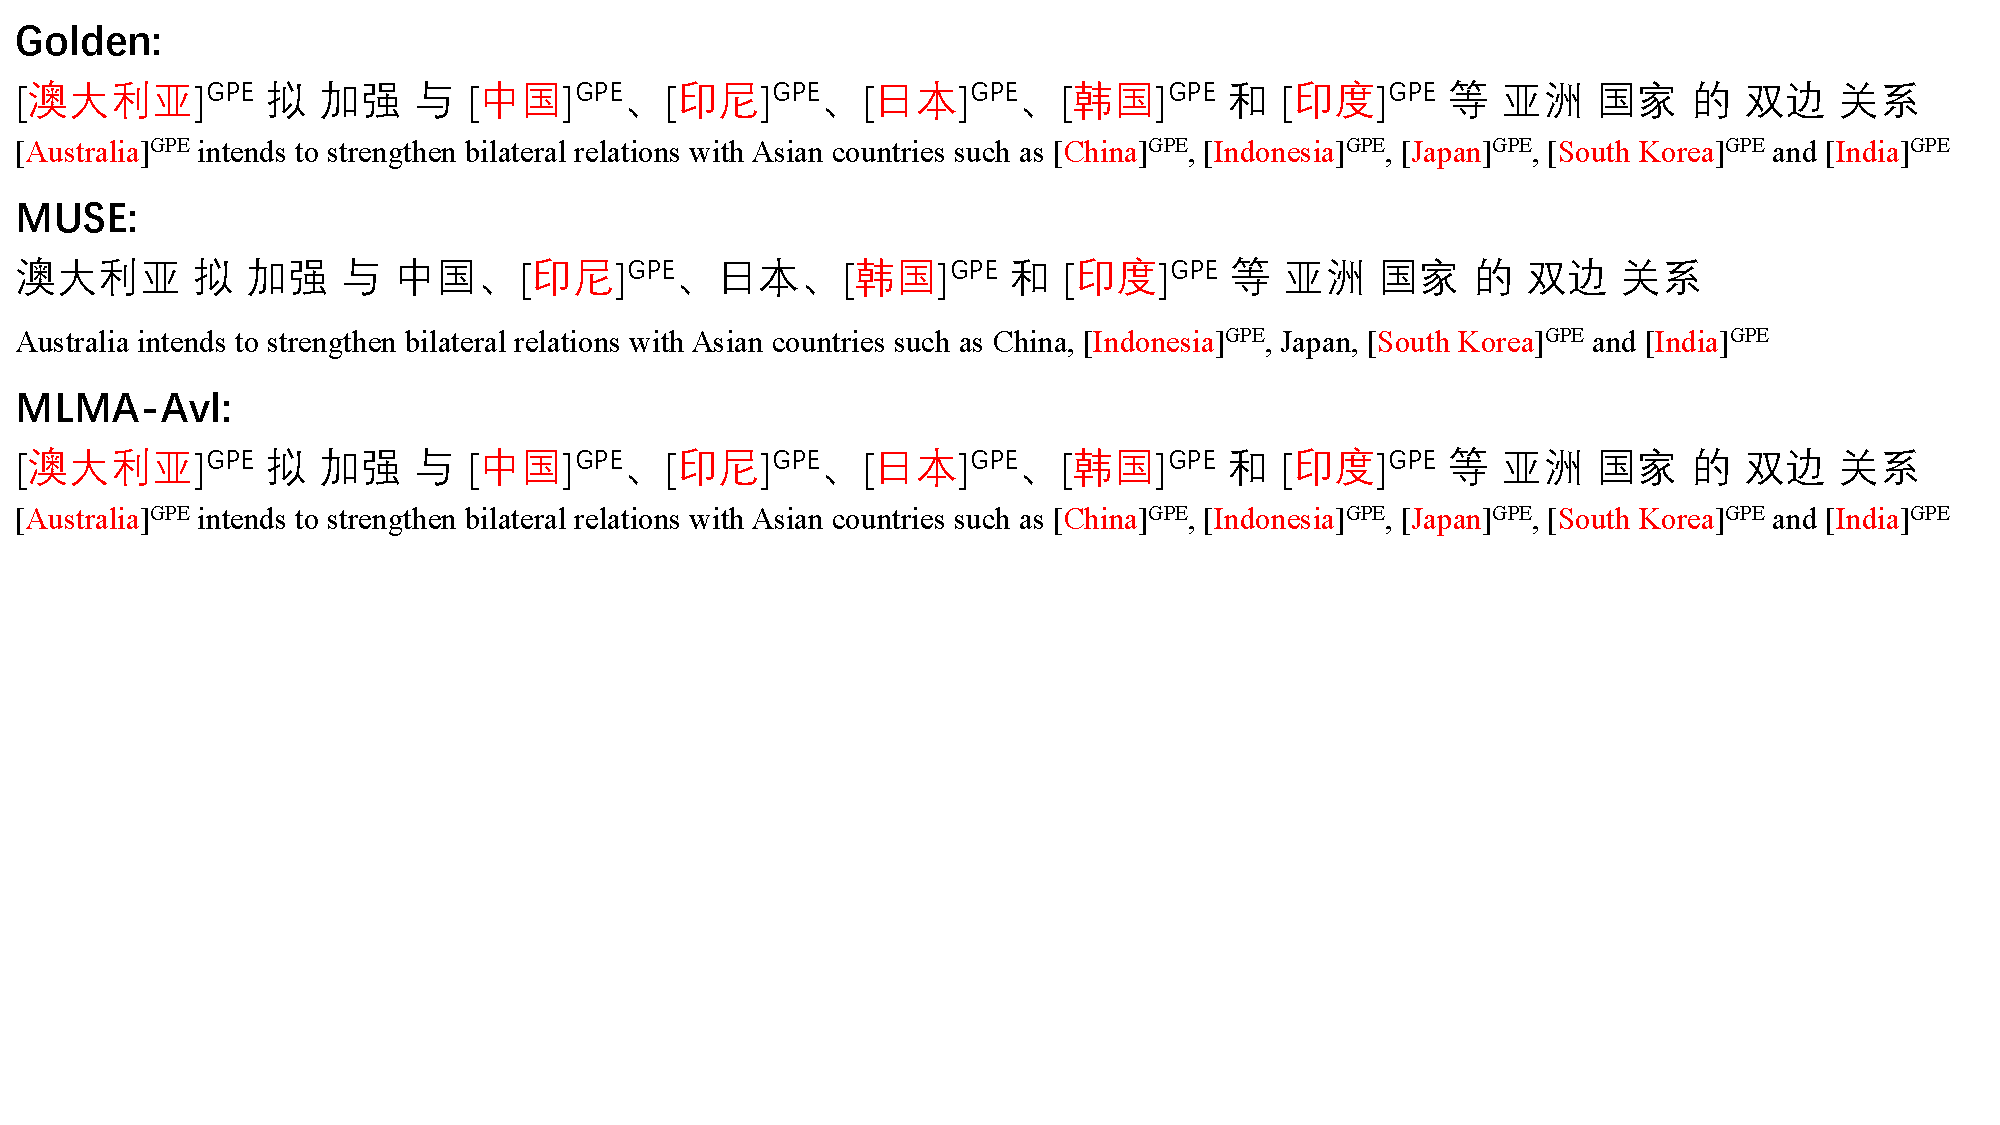
\includegraphics[trim=0.1cm 10.0cm 0.1cm %0cm,clip,width=0.8\textwidth]{zh_example.pdf}
	%	\caption{A case study of English-Chinese NER.}
	%	\label{fig:zh_example}
	%\end{figure*}

	\subsection{A Case Study of Chinese NER}
	%\footnote{Recent state-of-the-art methods did not release their code, so we cannot reproduce the performance of their approaches in this experiment.} 
	We conduct experiments and evaluate our approaches on a distant language pair, English-Chinese. The experiment results are shown in Table~\ref{table:NERchs}. \newcite{wang14cross} utilize 80K parallel sentences for annotation projection and report a strong performance.
	%\footnote{MUSE achieves extremely low performance when aligning from Chinese to English, we list their results of aligning from English to Chinese.}
	
	As Chinese and English do not share the alphabet, the number of identical strings is significantly smaller than similar languages pairs such as English-Spanish. Therefore, our token-based alignment method achieves a lower result comparing to MUSE which uses adversarial training. The MLMA-Avl method performs a direct alignment of internal representations and achieves a significant improvement over the token-based method. The initialization of CLWEs (init) also proves its effectiveness for distant language pairs by gaining further improvement and reaching a comparable result with \newcite{wang14cross}. This experiment suggests that cross-lingual transfer is still challenging between distant language pairs.
	
	%We further explore the differences between the MLMA-Avl and MUSE in this task. As shown in Fig~\ref{fig:zh_example}, MUSE adopts a word-level matching and fails to annotate some entities due to the distributions of entity names. While with the help of contextualized representations, the MLMA-Avl successfully recognizes the entities in a parallel pattern.
	
	%As shown in Fig~\ref{fig:zh_example}, the MLMA-Avl method successfully recognizes all entities in this sentence when MUSE fails. We hypothesize that the contextualized embeddings are enhanced with their surrounding entities, which makes them easier to be aligned to the embeddings of English entities.
	
    \begin{table*}[th]
		%\small
		\centering
		\begin{tabular}{l c c c c c c c c c c}% p{4cm}} 
			Model  & es & nl & de & da & el & it & pt & sv & Avg. \\% & Extra Resources\\
			\hline
			\newcite{das2011unsupervised}$\diamond$ & \textbf{84.2} & 79.5 & 82.8 & 83.2 & \textbf{82.5} & \textbf{86.8} & \textbf{87.9} & 80.5 & 83.31\\% & tbd\\
			%Tackstrom et al. (2013) & 87.1 & & & & & & &\\% & \\
			\newcite{fang2017model}$\dagger$ & 68.40 & 64.50 & 65.90 & 73.5 & 65.5 & 64.8 & 67.8 & 66.0 & 67.05 \\% & 20k dict.\\
			\newcite{fang2017model}$\dagger\ddagger$ & 81.20 & 82.30 & 78.90 & 81.9 & 80.1 & 81.9 & 82.1 & 78.1 & 80.81\\% & 20k dict, 1000 training tokens.\\
			MUSE* & 78.30  & 80.84  & 81.10  & 73.99  & 63.16  & 80.63  & 82.79  & 66.38 & 75.90\\% & None\\
			\hline
			\textit{Our methods} & & & & & & & &\\% & \\
			%Layer Align (Weighted Sum) & 79.70 ±  & 83.26 ±  & 85.35 ±  & None\\
			MLMA-Avl + f.w.s. & 81.20  & 85.54  & 84.92  & \textbf{83.45}  & 77.48  & 84.80  & 87.43  & 80.72 & 83.19 \\% & None\\
			MLMA-Avl + s.w.s. & 81.60  & 85.10  & 84.10  & 83.38  & 77.04  & 84.46  & 86.93  & \textbf{80.78} & 82.92 \\% & None\\
			MLMA-Avl (init) + f.w.s. & 82.27  & \textbf{85.97}  & \textbf{86.37}  & 82.25  & 81.31  & 86.28   & 86.53  & 80.00 & \textbf{83.87} \\% & None \\
			MLMA-Avl (init) + s.w.s. & 82.73  & 85.79  & 85.76  & 82.44  & 80.55  & 86.76  & 85.99  & 79.75 & 83.72 \\% & None \\
			\hline
		\end{tabular}
		\caption{ POS accuracy on test sets of European languages. The notations are consistent with Table~\ref{table:NERmain}. \newcite{fang2017model} report different results according to different resource requirements. We only list their best results in each setting. Methods with mark $\diamond$, $\dagger$, $\ddagger$ require parallel corpora, bilingual lexicons, and training data respectively.}
		\vspace{-1.5em}
		\label{table:POSmain}
	\end{table*}
	
	\subsection{Results for POS}
	We evaluate our methods on another sequence labeling task POS, and the results are shown in Table~\ref{table:POSmain}. We compare with previous studies using unsupervised cross-lingual clustering~\cite{fang2017model} and large-scale parallel corpora~\cite{das2011unsupervised}. As shown in Table~\ref{table:POSmain}, our models with deep semantic alignment outperform previous lexicon-based cross-lingual clustering by a large margin. When comparing to the previous method with a small amount of training data, the MLMA-Avl method obtains an improved accuracy without training data in the target languages.
	
	POS mainly relies on the information of each single word, and parallel corpora providing word alignment are effective for cross-lingual POS. Thus, previous annotation projection methods through parallel corpora are strong cross-lingual approaches for POS and often achieve a significantly better performance against previous unsupervised methods. The experimental results show that the proposed cross-lingual contextual representations are competitive and even achieve better average accuracy on these languages.
	
	\subsection{SWS v.s. FWS}
	As shown in Table~\ref{table:NERmain}, \ref{table:NERchs} and \ref{table:POSmain}, we observe that Self-Weighted Sum (SWS) methods generally outperform Fully-Weighted Sum (FWS) ones in NER tasks, while the opposite is true for POS tasks. Note that, SWS allows weights to vary at each position in a sequence, while FWS imposes adaptive weights for each hidden dimension. We hypothesize that NER is more context-sensitive and requires models to adapt to different context information, which makes SWS a better option. On the other hand, the part-of-speech of words is more independent across different context, but certain feature dimensions in contextualized representations may be critical for making a judgment. Therefore, FWS has the edge over SWS for its ability to select out these dimensions.
	
	\section{What is Connected during Alignment}
	In this section, we dive into our multilingual language model and investigate the question of what is connected between different languages during the alignment. From English 1B and Spanish Wikipedia, we randomly select 1,000 sentences for each language and extract their cross-lingual contextual representations using our MLMA-Avl model. We calculate the nearest neighbors in cosine distance for each word, and some of them are listed in Table~\ref{table:example}.
	\begin{table*}[th]
		\small
		\centering
		\begin{tabular}{p{4.2cm}|p{10.5cm}} 
			%\multicolumn{2}{l}{English words and their Top-5 nearest Spanish words accordings to MUSE} \\
			\hline
			\multicolumn{2}{l}{MUSE} \\
			\hline \hline
			\multicolumn{2}{l}{ brown:\ oliváceo (olive), negruzcas (blackish), negruzco (blackish), marrón (brown), ocráceo (ochraceous) } \\ % negruzca grisáceo pardo negruzcos blancuzcos \\
			\multicolumn{2}{l}{ chair:\ vicepresidenta (vice president), vicedecano (vice dean), cátedra (chair), vicedecana (vice dean), catedrático (professor) } \\ % emérito sillón vicerrector vicepresident catedrática \\
			\hline \hline
			\multicolumn{2}{l}{}\\	\multicolumn{2}{l}{}\\
			%Sentences from Enligsh  &  Sentences from Spanish\\
			\hline
			\multicolumn{2}{l}{MLMA-Avl} \\
			\hline \hline
			%brown neira 0.7786092164680399
			\multirow{2}{*}{\shortstack[l]{\textbf{[Brown]}'s office told news outlets \\ of his visit to Afghanistan ...}} & \textbf{[Neira]} escapó meses después rumbo a Miami para ... \\
			& (\textbf{Neira} escaped months later heading to Miami to ...) \\ \hline
			%brown verde 0.5239036231881408
			\multirow{2}{*}{\shortstack[l]{Wearing a \textbf{[brown]} suit with \\ matching hat, ...}} & La corona y vientre del macho son de un \textbf{[verde]} esmeralda brillante iridiscente, ...\\
			& (The crown and belly of the male are of an iridescent bright emerald \textbf{green}, ...) \\
			\hline \hline
			%chair asiento 0.6074887306147237
			\multirow{2}{*}{\shortstack[l]{Sweden currently holds \\ the EU \textbf{[chair]}.}} & Tras tomar posesión de su \textbf{[asiento]} , Lois decide limpiar el lago para empezar, ... \\
			& (After taking possession of her \textbf{seat}, Lois decides to clean the lake to begin, ... )\\ \hline
			%chair presidir 0.8963128369763216
			\multirow{2}{*}{\shortstack[l]{It's an honor to be asked to \\ \textbf{[chair]} the Man Booker Prize, ...}} &  ..., y fue la primera mujer en \textbf{[presidir]} un sindicato AFL-CIO. \\
			& (..., and was the first woman to \textbf{preside} over an AFL-CIO union.) \\
			\hline \hline
		\end{tabular}
		\caption{English words and their nearest Spanish words according to MUSE and MLMA-Avl.}
		\vspace{-1.5em}
		\label{table:example}
	\end{table*}
	
	In these cases, the multilingual language model can disambiguate word senses according to context information. For example, for a word ``brown" in English, the MLMA groups color ``brown" with ``verde" (green), and name ``Brown" with ``Neira" (a person's name in Spanish) in the Spanish corpus. Note that, our method is different from unsupervised translation in that instead of learning a precise matching between English and Spanish words, the multilingual language model establishes a high-level semantic connection between the source and the target language. The next example demonstrates that the MLMA is able to distinguish the part-of-speech of words. It connects an English verb ``chair" with a Spanish verb ``presidir" (preside), while a noun ``chair" with a noun ``asiento" (seat) in Spanish. To compare with unsupervised cross-lingual word embeddings, we list the top 5 similar words calculated using MUSE. As shown in Table~\ref{table:example}, MUSE successfully groups the English word ``brown" with Spanish words that are related to colors. However, without the help of contextual information, its ability of word sense disambiguation is limited. 
	
	\section{Related Work}
	\label{sec:related}
	Previous work in cross-lingual transfer learning can be roughly divided into two main branches: annotation projection and model transfer.
	%Our approach belongs to the Model Transfer.
	
	\subsection{Annotation Projection}
	\label{sec:annotation_projection}
	In annotation projection approaches, parallel or comparable corpora are commonly used \cite{yarowsky2001inducing,ehrmann11building,das2011unsupervised,li12joint,tackstrom2013token,wang14cross,ni17weakly}. The source language sentences of parallel corpora are first annotated either manually or by a pre-trained tagger. Then, annotations on the source side are projected to the target side through word alignment to generate distantly supervised training data. Finally, a model of the target language is trained on the generated data. Wikipedia contains multilingual articles for various topics and can thus be used to generate parallel/comparable corpora or even weakly annotated target language sentences~\cite{kim12multilingual}.
	
	However, parallel corpora and Wikipedia can be rare for true low-resource languages. \newcite{mayhew17cheap} reduce the resource requirement by proposing a cheap translation method, which ``translates" the training data from the source to the target language word by word through a bilingual lexicon. While \newcite{xie2018neural} reduce the requirement of bilingual lexicons by an unsupervised word-by-word translation through CLWEs.
	%\newcite{xie2018neural} further reduced the demand of lexicon by automatically learning a bilingual word mapping from unsupervised cross-lingual embeddings. 
	
	\subsection{Model Transfer}
	\label{sec:model_transfer}
	%Model Transfer method mainly learns a cross-lingual model based on language independent features, which enable the model trained on source language data to be directly applied to other languages.
	Model transfer methods train a model on the source language with language-independent features. Thus, the trained model can be directly applied to the target language.
	
	\newcite{McDonald11multi} design a cross-lingual parser based on delexicalized features like universal POS tags. \newcite{tackstrom12cross} reveal that cross-lingual word cluster features induced using large parallel corpora are useful. Lexicon and Wikipedia also demonstrate effectiveness for language-independent feature engineering.  \newcite{zirikly15cross} generate multilingual gazetteers from the source language gazetteers and comparable corpus. Page categories and linkage information to entries from Wikipedia are extracted as strong language-independent features (wikifier features)~\cite{tsai16cross}. \newcite{bharadwaj16phonologically} facilitate the cross-lingual transfer through phonetic features, which work well between languages like Turkish, Uzbek, and Uyghur, but are not strictly language independent. Recently, CLWEs are used as language-invariant representations for direct model transfer in NER~\cite{ni17weakly} and POS~\cite{fang2017model}.
	%Recently, \newcite{ni17weakly,fang2017model} use CLWEs as language-invariant representations for direct model transfer in cross-lingual NER and POS, respectively.
	%\newcite{ni17weakly} and \newcite{fang2017model}
	
	Some of the previous work also propose sequence labeling models with shared parameters between languages for performing cross-lingual knowledge transfer~\cite{lin18multi,cotterell17low,yang2017transfer,ammar16many,kim17cross}. However, these models are usually obtained through joint learning or multi-task learning and require annotated data from the target language.
	
	\section{Conclusion}
	In this paper, we focused on a low-resources cross-lingual setting and proposed transfer learning methods based on the alignment of deep semantic spaces between different languages. The proposed multilingual language model bridges different languages by automatically learning cross-lingual disambiguated representations. Abundant NER and POS experiments are conducted on the benchmark datasets. Experimental results show that our approaches using only monolingual corpora achieve improved performance comparing to previous strong cross-lingual studies with extra resources.
	
	\bibliography{acl2019}
	\bibliographystyle{acl_natbib}
\end{document}